\documentclass[tikz,border=4pt]{standalone}
\usetikzlibrary{positioning}

\begin{document}
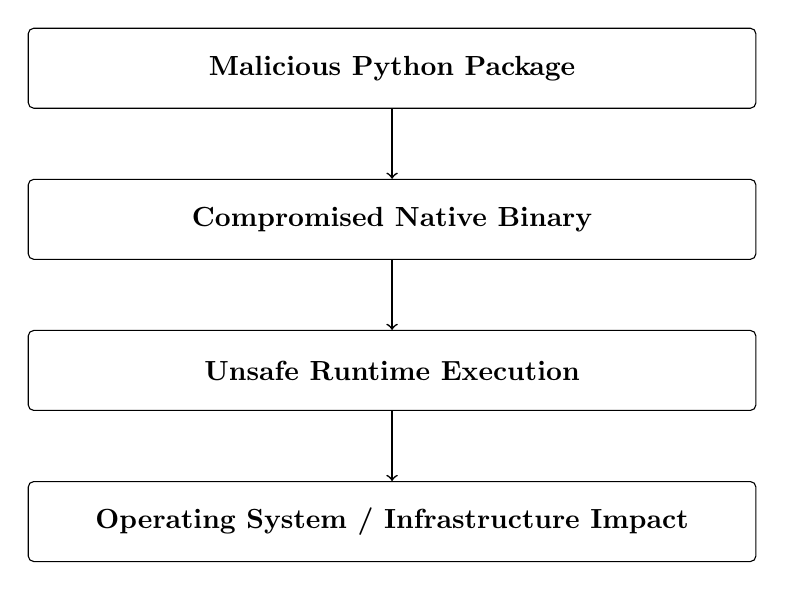
\begin{tikzpicture}[
  stage/.style={
    draw,
    rounded corners=2pt,
    text width=3.5in,
    minimum height=0.4in,
    align=center,
    font=\bfseries,
    inner sep=5pt
  },
  node distance=0.35in
]
\node[stage] (package) {Malicious Python Package};
\node[stage, below=of package] (binary) {Compromised Native Binary};
\node[stage, below=of binary] (runtime) {Unsafe Runtime Execution};
\node[stage, below=of runtime] (impact) {Operating System / Infrastructure Impact};

\draw[->, semithick] (package) -- (binary);
\draw[->, semithick] (binary) -- (runtime);
\draw[->, semithick] (runtime) -- (impact);
\end{tikzpicture}
\end{document}
